\documentclass[en,xcolor={dvipsnames,svgnames}]{beamer}

\usetheme{default}
\definecolor{bluehands-light}{HTML}{009BB4}
\definecolor{bluehands-dark}{HTML}{00243A}
\setbeamercolor*{structure}{bg=bluehands-dark,fg=bluehands-light}

\setbeamercolor*{palette primary}{use=structure,fg=white,bg=structure.fg}
\setbeamercolor*{palette secondary}{use=structure,fg=white,bg=structure.fg!75}
\setbeamercolor*{palette tertiary}{use=structure,fg=white,bg=structure.fg!50!black}
\setbeamercolor*{palette quaternary}{fg=white,bg=black}

\setbeamercolor{section in toc}{fg=black,bg=white}
\setbeamercolor{alerted text}{use=structure,fg=structure.fg!50!black!80!black}

\setbeamercolor{titlelike}{parent=palette primary,fg=structure.fg!50!black}
\setbeamercolor{frametitle}{bg=gray!10!white,fg=bluehands-light}

\setbeamercolor*{titlelike}{parent=palette primary}

\usepackage{appendixnumberbeamer}
\usepackage{pgfpages}
\usepackage{changepage}
\usepackage{csquotes}
\usepackage{scalerel, stackengine, amsmath, nccmath}
\usepackage{mathtools}
\usepackage{graphicx}
\usepackage{algorithm2e}
\usepackage{bm}
\usepackage{svg}
\usepackage{listings}
\usepackage[english, german]{babel}
%\usepackage{enumitem}
\usepackage{verbatim}

\usepackage{pgfkeys}
\pgfkeys{
	/padding/.is family, /padding,
	top/.estore in = \paddingtop,
	bottom/.estore in = \paddingbottom,
	left/.estore in = \paddingleft,
	right/.estore in = \paddingright,
	horizontal/.style = {left = #1, right = #1},
	vertical/.style = {top = #1, bottom = #1},
	default/.style = {horizontal = 0pt, vertical = 0pt}
}

\usepackage{tikz}
\usetikzlibrary{
	positioning,
	fit,
	calc,
	automata,
	math,
	decorations.pathreplacing,
	arrows.meta}
\tikzset{
	only/.code args={<#1>#2}{\only<#1>{\pgfkeysalso{#2}}},
	onslide/.code args={<#1>#2}{\onslide<#1>{\pgfkeysalso{#2}}},
}
\newcommand{\incslide}[1][1]{\tikzmath{
		\currentslide = \currentslide + #1;
		\nextslide = \currentslide + 1;}}
\newcommand{\kitbullet}{\raisebox{.2ex}{\KITmark}}

\newcommand{\bigitem}[1][0.08cm]{\vspace{#1}\item}
\newcommand{\wrapitem}[2][0.45\linewidth]{\parbox[t]{#1}{\strut #2\strut}}

\newcommand{\equalhat}{\mathrel{\stackon[1.5pt]{=}{\stretchto{%
				\scalerel*[\widthof{=}]{\wedge}{\rule{1ex}{3ex}}}{0.5ex}}}}
\newcommand{\ra}{\ensuremath{\Rightarrow}}
\newcommand{\arrowitem}{\item[\ra]}
\newcommand{\lookahead}[1]{
	\begin{itemize}
		\arrowitem #1 
	\end{itemize}
}
\newcommand{\hint}[1]{\item[~] \textit{#1}}
\newcommand{\keyword}[1]{\textcolor{blue}{\textbf{#1}}}
\newcommand<>{\notes}[1]{\note#2{
		\begin{adjustwidth}{-1.1cm}{-0.5cm}
			\begin{itemize}
				#1
			\end{itemize}
		\end{adjustwidth}
}}
\newcommand{\http}{\texttt{HTTP}}
\newcommand{\json}{\texttt{JSON}}

%\newcommand{\hint}[1]{\textit{#1}}

\newcommand{\leftgraphicswidth}{0.7\linewidth}
\newcommand{\rightnoteswidth}{0.29\linewidth}

\bibliographystyle{unsrt}
\setbeameroption{show notes on second screen=right}
\setbeamertemplate{bibliography entry title}{}
\setbeamertemplate{bibliography entry location}{}
\setbeamertemplate{bibliography entry note}{}
\setbeamersize
{
	text margin left=0.5cm,
	text margin right=0.5cm	
}

\DeclarePairedDelimiter\Bracket{\lbrack}{\rbrack}

\newenvironment{leftitemize}[1][7mm]{%
	\setlength{\leftmargini}{#1}
	\begin{itemize}
	}%
	{%
	\end{itemize}	
}
\newcommand{\leftitem}[1][1mm]{\item[\kitbullet\hspace*{-#1}]}
\newenvironment{conditions}[1][1]{%
	%	\newline \bigskip
	\begin{minipage}{#1\linewidth}
		%	\hspace{.2cm}
		\begin{tabular}{llc}
			\hspace{.6cm}&\hspace{1cm}&\\%\vspace{.5cm}\\
		}%
		{%
		\end{tabular}
	\end{minipage}%
}
\newcommand{\conditiontext}[1]{&\multicolumn{2}{l}{\kitbullet~~#1}\\}
\newcommand{\conditioneq}[1]{&&#1\\}

\title[Hyper Hypermedia]{Hyper Hypermedia - How much is the REST?}
\author{Jasper Park}
\institute[bluehands]{Bunte Nacht der Digitalisierung @ bluehands}
\logo{\includesvg[width=2.5cm,inkscapeformat=png]{../images/bluehands-logo}}

\date[07.06.24]{07. Juni 2024}

\begin{document}
	
	\begin{frame}
		\titlepage
		\notes{\item Hi \keyword{Jasper}}
	\end{frame}
	
	\begin{frame}
		Slides and code are available at\newline\newline
		https://github.com/park-jasper/bndd-hyper-hypermedia\newline
		
\includegraphics[width=0.5\textwidth]{../images/github_qr_code}
	\end{frame}
	
%	\begin{frame}
%		\begin{itemize}
%			\item REST Api \ra~json endpoint \ra~nice
%			\item[\ra] show json example
%			\item Wikipedia example: search, get result, start manipulating uri
%			\item[\ra] rather just (click) on the item
%			\item why not do that in API?
%			\item[\ra] enhance json
%			\item show backend c\# code how to define controller?
%			\item show frontend c\# code how to get content
%			\item somewhere: xml defined contract
%			\item live demo generic UI?
%		\end{itemize}
%	\end{frame}
	\begin{frame}
		\hspace{-0.54cm}
		
\includegraphics[height=\textheight]{../images/afraid_to_ask_hyper}
	\end{frame}
	\begin{frame}{Hypergraph}
		\vspace{-0.5cm}
		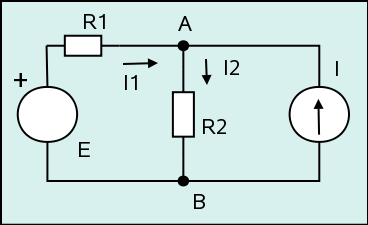
\includegraphics[width=0.9\textwidth]{../images/hypergraph_electric_circuit}
	\end{frame}
	\begin{frame}[fragile]{Hypertext}
		\texttt{HTTP \& HTML}
		\verbatiminput{../code/hypertext.html}
		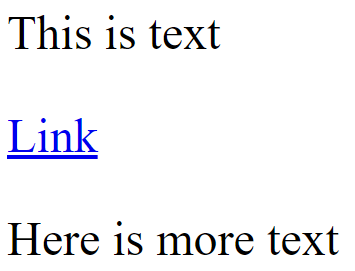
\includegraphics[height=0.3\textheight]{../images/hypertext.html}
	\end{frame}
	\begin{frame}
		\hspace{-0.54cm}
		
\includegraphics[height=\textheight]{../images/two_paths_cyoa}
	\end{frame}
	\begin{frame}{Hypermedia}
		\begin{itemize}
			\item \underline{Hyper}media describes any type of non-linear media
			\item Text
			\item Images
			\item Sound / Video
		\end{itemize}
	\end{frame}
	\begin{frame}{How much is the \{REST\} - REST maturity model}
		\begin{itemize}
			\item Level 0: The Swamp of POX (Plain Old XML)
			\only<1>{\newline
			Using \http, a single endpoint, result depends on the parameter
			}
			\item Level 1: Resources
			\only<2>{\newline
			Multiple endpoints are available to call
			}
			\only<1-7>{\item Level 2: Methods}
			\only<8->{\item Level 2: Methods, Headers, Query Parameters, Status Codes}
			\only<3-4>{\newline
			Call the same endpoint with different \http~verbs:\newline
			\texttt{GET, POST, PUT, PATCH, DELETE}\onslide<4>{\texttt{, HEAD, OPTIONS}}
			}
			\only<5-7>{
				\begin{itemize}
					\only<5-7>{\item Level 2.1: Headers}
					\only<6-7>{\item Level 2.2: Query Parameters}
					\only<7>{\item Level 2.3: Status Codes}
				\end{itemize}
				}
		
			\item Level 3: Hypermedia Controls
			\only<8>{\newline
			Content Negotiation:\newline
			\texttt{Accept \& Content-Type: application/json}\newline\newline
			Hypermedia As The Engine Of Application State (\texttt{HATEOAS})
			}
		\end{itemize}
	\end{frame}
	\begin{frame}[fragile]{HATEOAS: Linking related Resources}
		\only<1>{
		Level 2 response \json
		\verbatiminput{../code/rest.json}
		}
		\only<2>{
		Level 3 response \json
		{\smaller
			\verbatiminput{../code/hypermedia.json}
		}
		}
	\end{frame}
	\begin{frame}
		\hspace{-0.54cm}
		
\includegraphics[height=\textheight]{../images/drake_meme_client_urls}
	\end{frame}
	
	\begin{frame}{HATEOAS: Actions}
		\smaller
		\verbatiminput{../code/hypermedia-actions.json}
	\end{frame}
	\begin{frame}
		\hspace{-0.54cm}
		
\includegraphics[height=\textheight]{../images/ggg_actions}
	\end{frame}
	
%	\begin{frame}{API example: Uni lecture and exam backend}
%		\begin{itemize}
%			\item \texttt{GET /lectures}
%			\item \texttt{GET /lecture/\{name\}/\{year\}}
%			\item \texttt{GET /exam/\{lecture\}/\{year\}}
%			\item \texttt{POST /exam/\{lecture\}/\{year\}/register}
%			\item \texttt{POST /exam/\{lecture\}/\{year\}/unregister}
%			\item \texttt{POST /exam/\{lecture\}/\{year\}/change-grade}
%		\end{itemize}
%	\end{frame}
%	\begin{frame}[fragile]
%		Lecture:
%		\begin{lstlisting}
%{
%	"name": "Statistics 1",
%	"year": 2024,
%	"lecturer": "Jane Doe"
%}
%		\end{lstlisting}
%		Exam:
%		\begin{lstlisting}
%{
%	"lecture": "Statistics 1",
%	"year": 2024,
%	"grade": null
%}
%		\end{lstlisting}
%	\end{frame}
	\begin{frame}
		
\includegraphics[width=0.9\textwidth]{../images/generate_everything_from_contract}
	\end{frame}
	\begin{frame}{XMLContract}
		\smaller
		\verbatiminput{../code/bndd-hypermedia/Hypermedia-Bndd-Reduced.xml}
	\end{frame}
\end{document}